% 隔離テスト用ドライバ: 10-separation-strategy のみを単独ビルド（共有 main.tex に影響しない）
% フレーム番号10に偽装して帯色(barC)とセクション名を本番と一致させる。
\documentclass[11pt,aspectratio=43,dvipsnames]{beamer}
\usepackage{luatexja}
\usepackage[match]{luatexja-fontspec}
\setmainjfont{HaranoAjiGothic}
\setsansjfont{HaranoAjiGothic}
\renewcommand{\kanjifamilydefault}{\gtdefault}
\usepackage{amsmath, amssymb}
\usepackage[version=4]{mhchem}
\usepackage{booktabs}
\usepackage{multirow}
\usepackage{colortbl}
\usepackage{graphicx}
\graphicspath{{figures/}}
\usepackage{pgfplots}
\pgfplotsset{compat=1.18}
% =====================================================================
%  seminar テーマ定義（既存 Marp デザインの Beamer 再現）
%  ・濃青の恒常ヘッダーバー（セクション名＋ページ番号）
%  ・専用表紙（アクセントライン＋グラデ背景）
%  ・本文は白地・濃青見出し
%  main.tex から \input する（パッケージではなく生プリアンブル）
% =====================================================================

% ---- ベース：装飾の少ないテーマから組む -----------------------------
\usetheme{default}
\usefonttheme{professionalfonts}
\setbeamertemplate{navigation symbols}{}   % ナビゲーション記号を消す

% ---- TikZ（ヘッダー・表紙・矢印などで使用）-------------------------
\usepackage{tikz}
\usetikzlibrary{arrows.meta, positioning, calc, shapes.geometric, fit, patterns}

% ---- 配色（ルール準拠）---------------------------------------------
\definecolor{HeaderBlue}{HTML}{0f5a7a}   % ヘッダー・見出しの濃青
\definecolor{DateGray}{HTML}{334b5e}     % 表紙の日付グレー
\definecolor{TitleBG}{HTML}{edf5fb}      % 表紙グラデの薄青

% コンテンツ用パレット（図・ハイライト・矢印で共通利用）
\definecolor{ArrowBlue}{HTML}{1F6FC4}    % 矢印・強調の青
\definecolor{HiPink}{HTML}{F4B6BE}       % ハイライト見出し（暖色）
\definecolor{HiBlue}{HTML}{C7DCEF}       % ハイライト見出し（寒色）
\definecolor{IpaBlue}{HTML}{1F5FC4}      % グラフ系列1（青）
\definecolor{DipeOrange}{HTML}{E8821E}   % グラフ系列2（橙）
\definecolor{SpRed}{HTML}{C0392B}        % 反応式：プロピレン強調の赤
\definecolor{SpBlue}{HTML}{1F6FC4}       % 反応式：エテン・エタン・CH0.5 の青

% 帯（ヘッダーバー）のパート別配色（寒色グラデ）。本文枠線は HeaderBlue のまま。
%  1-4 導入・全体像／5-9 反応・反応器／10-13 分離／14-17 最適化・経済・結言
\definecolor{barA}{HTML}{0F5A7A}   % 1-4  青緑
\definecolor{barB}{HTML}{1D6E6E}   % 5-9  シアン寄り
\definecolor{barC}{HTML}{2E4C8A}   % 10-13 青
\definecolor{barD}{HTML}{4A3C84}   % 14-17 紫

\setbeamercolor{normal text}{fg=black, bg=white}
\setbeamercolor{frametitle}{fg=HeaderBlue, bg=white}
\setbeamercolor{itemize item}{fg=HeaderBlue}
\setbeamercolor{itemize subitem}{fg=HeaderBlue}
\setbeamercolor{block title}{fg=white, bg=HeaderBlue}
\setbeamercolor{block body}{fg=black, bg=TitleBG}
\setbeamercolor{alerted text}{fg=HeaderBlue}

% ---- フォントサイズ（Marp px をおおよそ pt に対応）------------------
\setbeamerfont{frametitle}{size=\large, series=\bfseries}   % スライド見出し ~44px

% ---- 恒常ヘッダーバー（headline）-----------------------------------
%  左：セクション名（無ければロゴ枠）／右：ページ番号
\newcommand{\HeaderLogo}{}   % ロゴを入れるなら \renewcommand で画像指定
% 本線の総枚数（分母）。appendix に入ると分子がこれを超え、本線/付録を見分けられる。
\newcommand{\MainTotal}{17}
% パート別に帯色を選ぶ：1-4=barA／5-9=barB／10-13=barC／14-17=barD。
% スライド4の独自帯（CC・GCC）など headline を上書きする箇所でも呼べるよう独立コマンド化。
% 併せて本文アクセント色 HeaderBlue 自体をそのパート色へ再定義し、各スライドの
% 図・枠線・矢印・ボックス（HeaderBlue 参照）をパート色に連動させる（\colorlet は大域的）。
% headline はフレーム本文より前に組まれるため、ここでの再定義が本文に効く。
\newcommand{\SetBarColor}{%
  \ifnum\insertframenumber<5\setbeamercolor{headerbar}{fg=white, bg=barA}\colorlet{HeaderBlue}{barA}%
  \else\ifnum\insertframenumber<10\setbeamercolor{headerbar}{fg=white, bg=barB}\colorlet{HeaderBlue}{barB}%
  \else\ifnum\insertframenumber<14\setbeamercolor{headerbar}{fg=white, bg=barC}\colorlet{HeaderBlue}{barC}%
  \else\setbeamercolor{headerbar}{fg=white, bg=barD}\colorlet{HeaderBlue}{barD}%
  \fi\fi\fi}
\setbeamertemplate{headline}{%
  \ifnum\insertframenumber>0\relax
    \SetBarColor
    \begin{beamercolorbox}[wd=\paperwidth, ht=4.5ex, dp=1.8ex,
                           leftskip=1.2em, rightskip=1.2em]{headerbar}%
      \color{white}\bfseries\large
      \insertsectionhead%
      \hfill
      \insertframenumber/\MainTotal%
    \end{beamercolorbox}%
  \fi
}
\setbeamercolor{headerbar}{fg=white, bg=barA}
\setbeamertemplate{footline}{}             % フッターは使わない
\setbeamersize{text margin left=3mm, text margin right=3mm}  % 本文を横幅ぎりぎりまで

% 【必須ルール】帯と本文の間の余白を詰める（全スライド共通）。
%  beamer 既定の天井スキップで本文が帯から離れるのを、headline 直後の負スキップで打ち消す。
%  情報量最優先：無駄な上余白は作らない。各スライドは [t] 推奨。
\addtobeamertemplate{headline}{}{\vskip-2.6ex}

% frametitle はバーの直下に置く（左寄せ・濃青・太字）
\setbeamertemplate{frametitle}{%
  \vskip0.6ex
  \hspace{0.6em}\usebeamerfont{frametitle}\usebeamercolor[fg]{frametitle}\insertframetitle\par
  \vskip0.2ex
}

% ---- 箇条書きをシンプルに ------------------------------------------
\setbeamertemplate{itemize item}{\textbullet}
\setbeamertemplate{itemize subitem}{--}

% =====================================================================
%  再利用ヘルパー（どのスライドでも使える共通部品）
% =====================================================================
% 青い矢印 →（行中に置ける。結論や対応関係の明示に）
\newcommand{\bluearrow}{\tikz[baseline=-0.5ex]\draw[ArrowBlue, line width=1pt,
  -{Stealth[length=2.2mm]}] (0,0)--(0.55,0);}

% ハイライト見出し  \hilite{色}{テキスト}  例: \hilite{HiPink}{IPA選択率の温度依存性}
\newcommand{\hilite}[2]{\colorbox{#1}{\bfseries\normalsize #2}}

% パラメータ表  \paramtable{ 項目 & 値 \\ ... }  （左:項目 右:値、単位は数式推奨）
\newcommand{\paramtable}[1]{%
  {\footnotesize\renewcommand{\arraystretch}{1.15}%
   \begin{tabular}{@{\hspace{1em}}ll@{}}#1\end{tabular}}}

% =====================================================================
%  専用表紙コマンド  \seminartitlepage
%  ルール準拠：アクセントライン(120x8px相当) + 160度グラデ背景
%               h1 60px / h2 34px濃青 / 著者27px / 日付22pxグレー
%  使い方: \title{} \subtitle{} \author{} \date{} を設定後に呼ぶ
% =====================================================================
\newcommand{\seminartitlepage}{%
  \begin{frame}[plain]
    \begin{tikzpicture}[remember picture, overlay]
      % 背景グラデ（左上 薄青 → 右下 白、斜め）
      \shade[top color=TitleBG, bottom color=white, shading angle=20]
        (current page.south west) rectangle (current page.north east);
      % アクセントライン（上から少し下げて左に）
      \fill[HeaderBlue]
        ([xshift=9mm, yshift=-12mm]current page.north west)
        rectangle ++(16mm, 1.1mm);
      % テキストブロック（左寄せ・縦中央付近）
      \node[anchor=center, text width=0.86\paperwidth, align=center]
            at (current page.center) {%
        {\fontsize{22pt}{28pt}\selectfont\bfseries\color{black}\inserttitle\par}
        \vspace{0.3em}
        {\fontsize{16pt}{20pt}\selectfont\bfseries\color{HeaderBlue}\insertsubtitle\par}
        \vspace{1.0em}
        {\fontsize{13pt}{17pt}\selectfont\color{black}\insertauthor\par}
        \vspace{0.4em}
        {\fontsize{11pt}{14pt}\selectfont\color{DateGray}\insertdate\par}
      };
    \end{tikzpicture}
  \end{frame}
}

\begin{document}
\setcounter{framenumber}{9}
\section{分離戦略}
% =====================================================================
%  10  分離戦略 — 左=分離の考え方（タイトル付き説明＋沸点マップ）｜右=工程フロー＋膜有無比較
%  source_memo: trial #201・07章 Table7.1/Fig7.1。分離目標(要求純度)を主役に:
%   C3H6 99.5wt%(α≈1.07)・H2 99.9mol%。脱ブタン=C4除去、脱エタン=軽質分離。
%   膜有無比較(共通フィード C3H6 60.7mol%): 膜+塔 TAC135/117段/94m vs 塔単独 TAC1625/200段/156m。
%  方針：まず左で「沸点→分離操作」の考え方を示し、右で工程フローと膜の効果へ。
%        左右は全高の仕切りで分ける。重なり・はみ出し・無駄余白なし。丸括弧禁止。
% =====================================================================
\definecolor{SepGreen}{HTML}{2E9E5B}
\begin{frame}[t]

  \vspace{0.05em}

  \begin{columns}[T,onlytextwidth]
    % ===== 左：分離の考え方（タイトル付き説明＋沸点マップ）｜右端に全高の仕切り =====
    \begin{column}{0.34\textwidth}
      \resizebox{!}{\dimexpr\textheight-6mm\relax}{%
      \begin{tikzpicture}[
        x=1cm, y=1cm, >=Stealth, font=\small,
        cut/.style={dashed, HeaderBlue, line width=0.8pt, -{Stealth[length=2mm]}},
        cuthard/.style={dashed, SpRed, line width=1.1pt, -{Stealth[length=2.2mm]}},
        tick/.style={HeaderBlue, line width=0.8pt},
        lab/.style={anchor=west, font=\small\bfseries},
        cmp/.style={anchor=west, font=\small},
        val/.style={anchor=east, font=\footnotesize, text=black!55},
      ]
        \useasboundingbox (-0.7,-0.9) rectangle (4.55,10.7);
        % --- 全高の仕切り縦線（右端：右の工程と分ける）---
        \draw[black!35, line width=0.9pt] (4.35,-0.8) -- (4.35,10.6);
        % --- タイトル付き説明 ---
        \node[anchor=north west, font=\large\bfseries, text=HeaderBlue] at (-0.6,10.5) {分離の考え方};
        \node[anchor=north west, font=\normalsize, text width=4.6cm, align=left] at (-0.6,9.7)
          {成分を沸点順に並べ、各境界に分離操作を割り当てた。沸点差の大きい境界は蒸留、沸点差 $6$ K と小さい C3 対のみ膜＋蒸留で分離。};
        % --- 沸点マップ（軸＝上が高沸点）---
        \draw[HeaderBlue, line width=1.3pt, ->] (0.3,0.5) -- (0.3,7.15);
        \node[anchor=west, font=\footnotesize, text=black!60] at (0.5,6.98) {[$^\circ$C]};
        \foreach \y/\name/\bp in {6.7/{$\mathrm{C_4H_{10}}$}/{$-1$}, 3.9/{$\mathrm{C_2H_6}$}/{$-89$}, 2.6/{$\mathrm{CH_4}$}/{$-161$}, 1.0/{$\mathrm{H_2}$}/{$-253$}}{
          \draw[tick] (0.15,\y) -- (0.45,\y);
          \node[cmp] at (0.5,\y) {\name};
          \node[val] at (0.0,\y) {\bp};
        }
        % C3 ペア（赤・近接）
        \draw[tick, SpRed] (0.15,5.5) -- (0.45,5.5);
        \draw[tick, SpRed] (0.15,5.1) -- (0.45,5.1);
        \node[cmp, text=SpRed] at (0.5,5.5) {$\mathrm{C_3H_8}$};
        \node[cmp, text=SpRed] at (0.5,5.1) {$\mathrm{C_3H_6}$};
        \node[val, text=SpRed] at (0.0,5.5) {$-42$};
        \node[val, text=SpRed] at (0.0,5.1) {$-48$};
        % cuts（境界ごとの分離操作）
        \draw[cut] (0.3,6.1) -- (1.9,6.1);
        \node[lab] at (2.0,6.1) {脱ブタン};
        \draw[cuthard] (0.3,5.3) -- (1.9,5.3);
        \node[lab, text=SpRed] at (2.0,5.3) {膜＋蒸留};
        \node[anchor=west, font=\footnotesize, text=SpRed] at (2.0,4.9) {沸点差 6 K};
        \draw[cut] (0.3,4.5) -- (1.9,4.5);
        \node[lab] at (2.0,4.5) {脱エタン};
        \draw[cut] (0.3,1.8) -- (1.9,1.8);
        \node[lab] at (2.0,1.8) {PSA};
        % --- マップのタイトル（最下部）---
        \node[anchor=north, font=\large\bfseries] at (1.8,-0.15) {沸点と分離操作};
      \end{tikzpicture}}
    \end{column}

    % ===== 右：工程フロー（上）＋膜有無の比較（下）=====
    \begin{column}{0.63\textwidth}
      % --- 上：横向き工程フロー（分離ブロックを緑・大きく強調）---
      \resizebox{\linewidth}{!}{%
      \begin{tikzpicture}[
        x=1cm, y=1cm, >=Stealth, font=\small,
        sep/.style={draw=SepGreen, line width=1.4pt, fill=SepGreen!22, rounded corners=3pt, align=center,
                    inner sep=2pt, minimum width=1.75cm, minimum height=1.05cm, font=\normalsize\bfseries},
        rxn/.style={draw=black, fill=white, rounded corners=2pt, align=center,
                    inner sep=2pt, minimum width=1.3cm, minimum height=0.72cm, font=\small\bfseries},
        raw/.style={align=center, font=\small\bfseries},
        goalC/.style={draw=SpRed, line width=1.2pt, fill=SpRed!12, rounded corners=3pt,
                      align=center, inner sep=4pt, text=SpRed},
        goalH/.style={draw=HeaderBlue, line width=1.2pt, fill=HiBlue!55, rounded corners=3pt,
                      align=center, inner sep=4pt},
        sub/.style={align=center, font=\scriptsize, text=black!60},
        main/.style={-{Stealth[length=2.8mm]}, HeaderBlue, line width=1.6pt},
        br/.style={-{Stealth[length=2.2mm]}, black!70, line width=1.1pt},
      ]
        % 主フロー（分離=緑で大きく、反応器=小さめ青）
        \node[raw] (raw) at (0.0,3.0) {原料\\LPG};
        \node[sep] (deb) at (2.0,3.0) {脱ブタン};
        \node[rxn] (rx)  at (4.0,3.0) {反応器};
        \node[sep] (de)  at (6.0,3.0) {脱エタン};
        \node[sep] (mc)  at (8.1,3.0) {膜＋蒸留};
        \node[goalC] (prod) at (10.8,3.0)
          {$\mathrm{C_3H_6}\!\mid\!\mathrm{C_3H_8}$\\[1pt]{\Large\bfseries 99.5 wt\%}};
        \draw[main] (raw) -- (deb);
        \draw[main] (deb) -- (rx);
        \draw[main] (rx) -- (de);
        \draw[main] (de) -- (mc);
        \draw[main] (mc) -- (prod);
        % PSA 枝（上）＋ H2 目標
        \node[sep, minimum width=1.3cm] (psa) at (6.0,5.2) {PSA};
        \draw[br] (de.north) -- node[left, font=\scriptsize]{軽質} (psa.south);
        \node[goalH] (h2) at (8.5,5.2)
          {$\mathrm{H_2}\!\mid\!$軽質\\[1pt]{\Large\bfseries 99.9 mol\%}};
        \draw[br] (psa.east) -- (h2.west);
        % 除去・循環（下、補助）
        \node[sub] (c4) at (2.0,1.35) {$\mathrm{C_4}$ 除去};
        \draw[br, black!55] (deb.south) -- (c4.north);
        \node[sub] (rec) at (8.1,1.35) {$\mathrm{C_3H_8}$ 循環};
        \draw[br, black!55] (mc.south) -- (rec.north);
      \end{tikzpicture}}

      \vspace{0.1em}

      % --- 下：膜有無の比較（レポート Fig7.1 形式のままスライド用に拡大）---
      \centering
      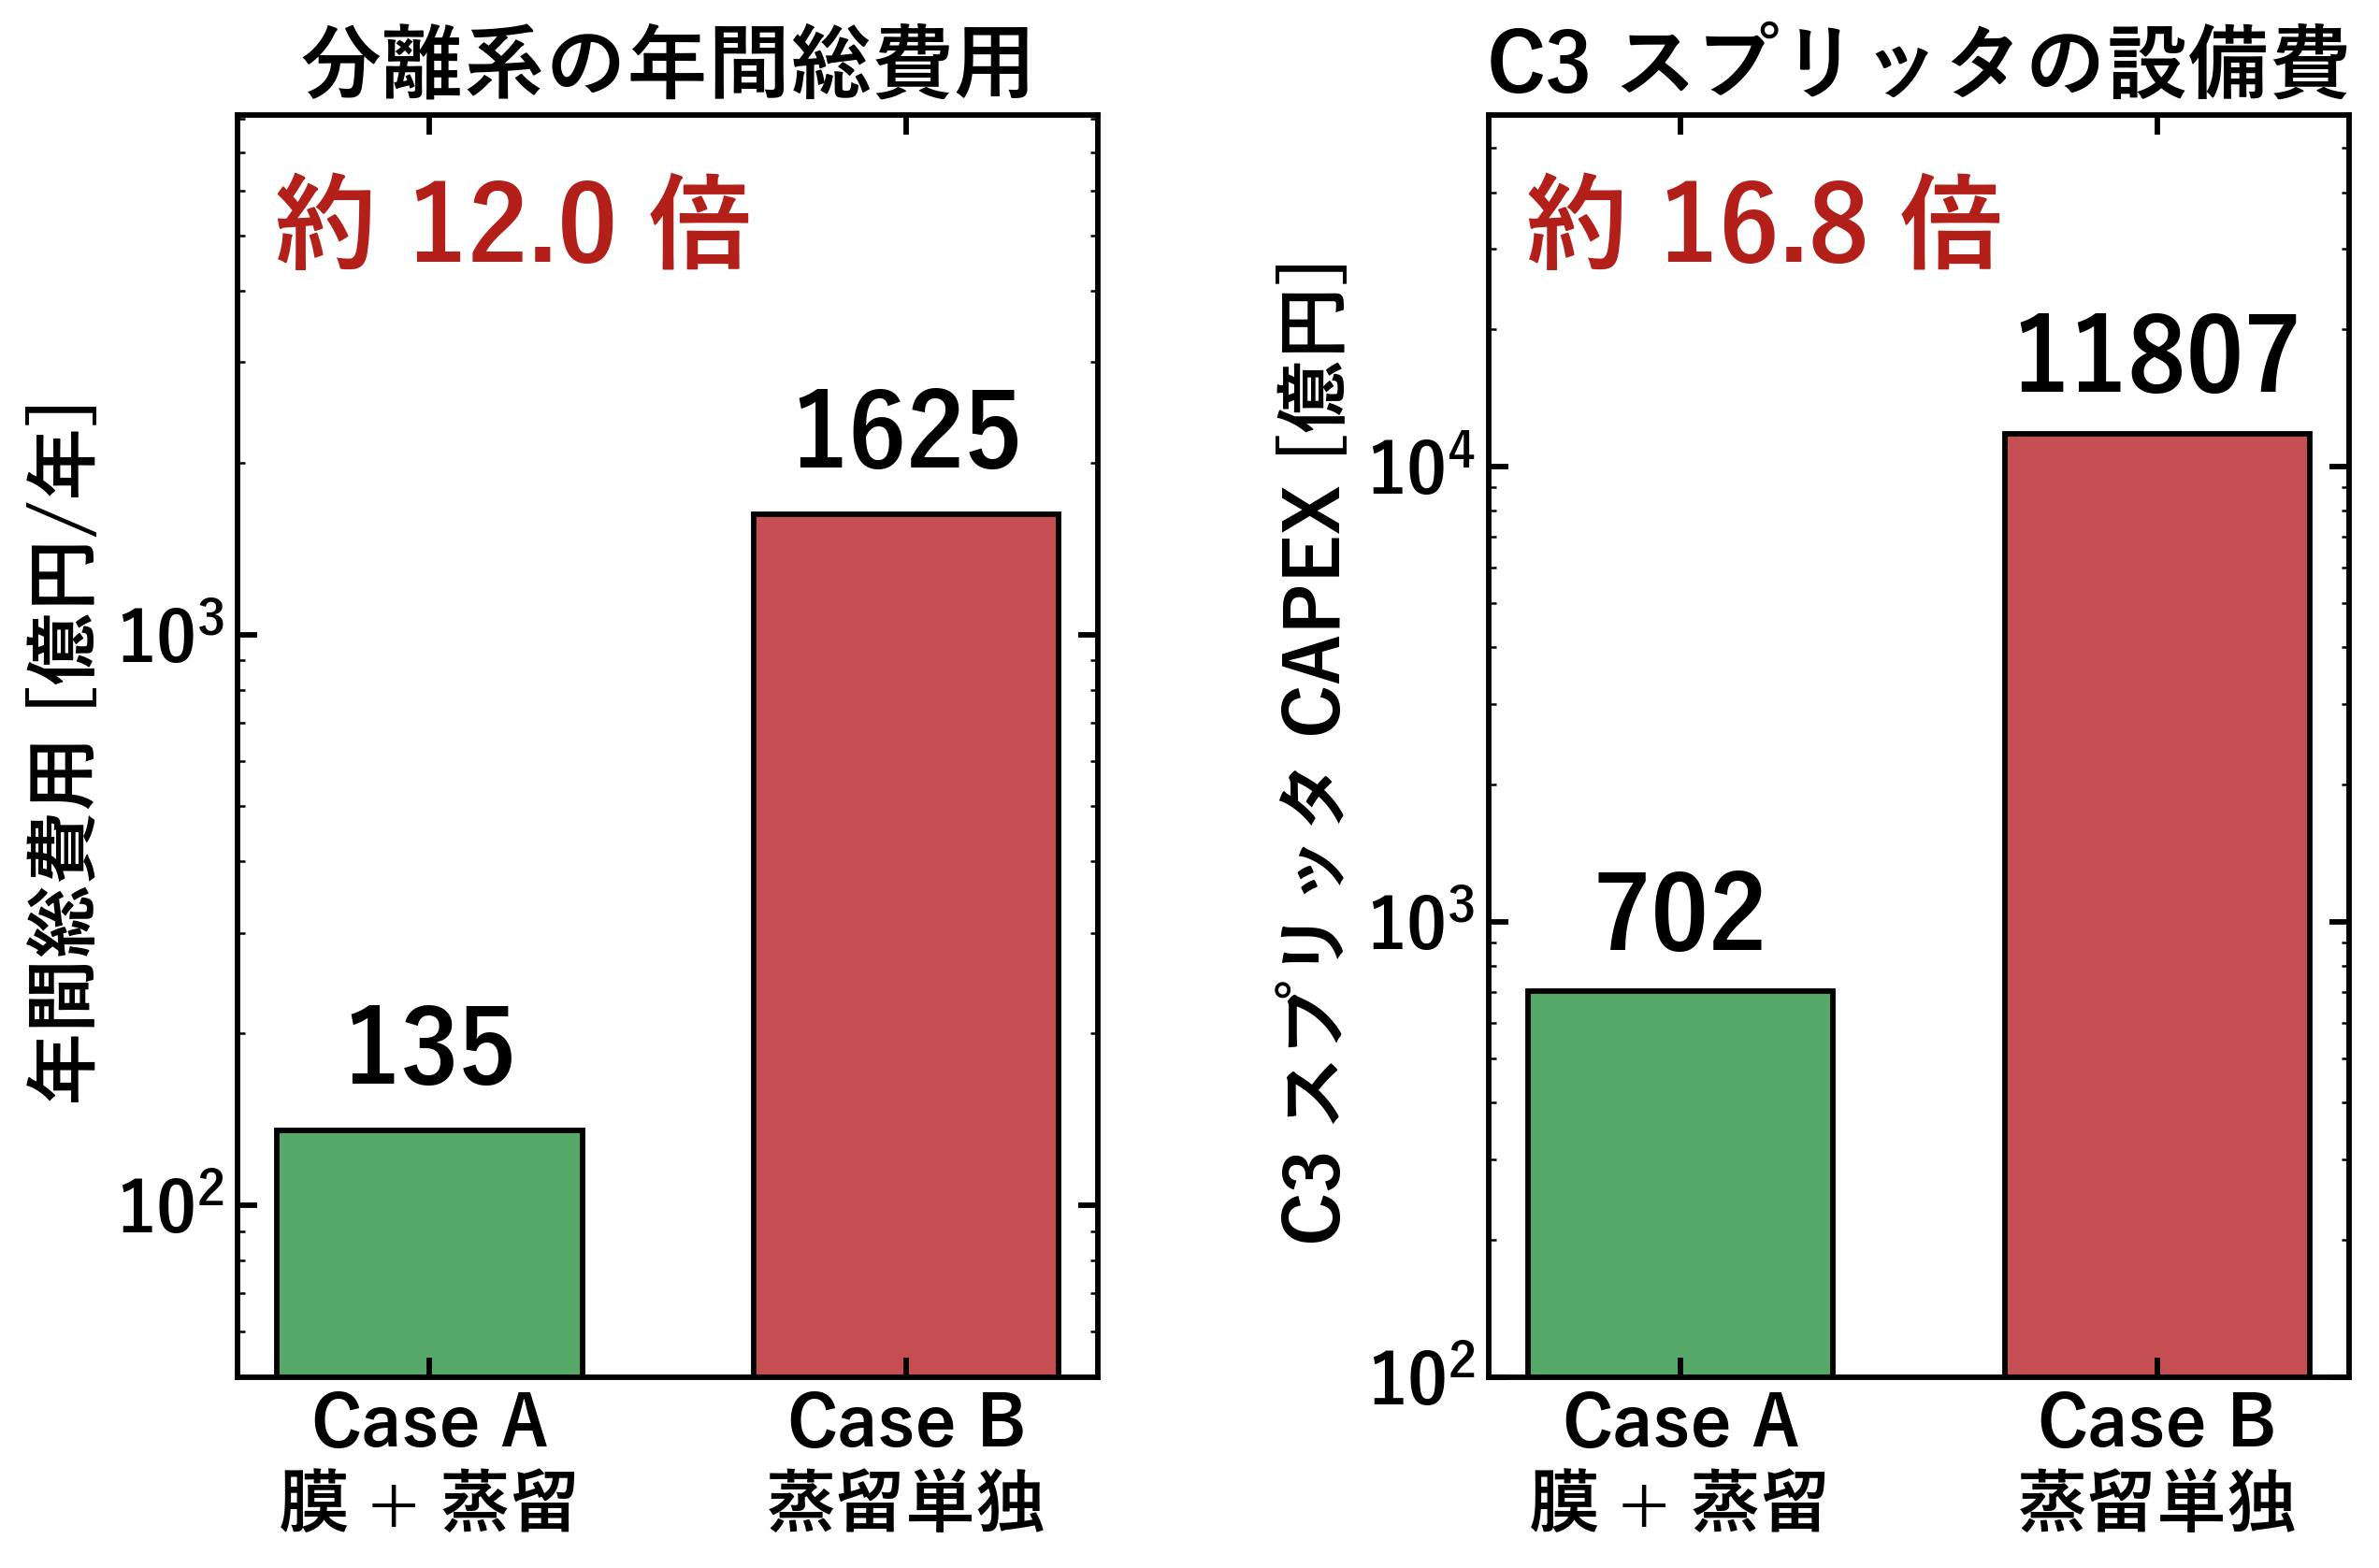
\includegraphics[width=\linewidth]{membrane_vs_dist3_slide}\par
      \vspace{0.08em}
      \raggedright
      {\scriptsize 膜無しは塔単独で $200$ 段・塔高 $156$ m を要する。}
    \end{column}
  \end{columns}

\end{frame}

\end{document}
